\chapter{Tasks, architectures, and data sets}
\label{chap:theory}

In this chapter, we give a brief overview of the theoretical foundations necessitated for this thesis. First, we define the main tasks that are part of the solution. Moreover, we describe the utilized neural network architectures. Lastly, we describe used data sets and introduce evaluation metrics.

\section{Automatic Speech Recognition}

Automatic Speech Recognition (ASR) is one of the most popular tasks in NLP, and without a doubt, it is one of the most important ones. With ever-growing technology that becomes more and more integrated with our day-to-day life, it is clear that ASR will take an essential role in this process.

In this section, we first briefly examine the history and then describe the most popular contemporaneous approaches for ASR.

\subsection{Brief history}

The first attempts for ASR systems stem from the 1950s. At that time, researchers focused their interest on acoustics-phonetics, which describes phonetic elements of speech, including phonemes \parcite{juang2005automatic}. The first ASR system worked with syllables, vowels, and phonemes. An example can be taken spoken digit recognizer from Bell laboratories. Their system estimated formant frequencies (as a vowel is pronounced, vocal tract sounds with natural modes of resonance called formant) of vowel regions of an isolated digit. 

A big leap in ASR systems was the introduction and popularization of Hidden Markov models (HMMs) in the 1980s. HMMs caused architecture to shift from pattern recognition to statistical modeling. The success of HMM-based ASR systems continues even today in the form of hybrid models consisting of HMMs and either Gaussian Mixture Models (GMMs) or Artificial Neural Networks (ANNs).

In the last few years, deep neural networks gained much popularity. In many tasks, ranging from image processing to natural language processing, DNNs outperformed other known methods. Besides their performance, they tend to require less expertise and engineering skills for a particular task than other methods. This makes them available for researchers in many areas. DNNs are becoming a standard in ASR currently, but the first attempts were already made briefly after the introduction of the backpropagation algorithm \parcite{rumelhart1986learning}. They were used for recognition of phonemes \parcite{waibel1989phoneme} or few words \parcite{lubensky1988learning}. Further important milestones for ASR in the 2010s were recurrent neural networks and attention (applied, for example, in \perscite{chorowski2014end}) in the 2010s.

\subsection{Models}
In this section, we introduce contemporary models utilized for ASR. There are two such approaches: (1) HMM-based models, (2) End-to-End neural models.

\subsubsection{HMM-based models}
HMMs (Hidden Markov Models) are probably the most used technique in ASR \parcite{padmanabhan2015machine}. HMMs are in the ASR context used with either GMMs (Gaussian Mixture Models)  or ANNs (Artificial Neural Networks).  Practitioners often refer to the HMM-based models as a hybrid.

A typical pipeline of an HMM-based model works as follows: the input is first pre-processed and converted to features, typically the MFCCs (see \cref{mfcc}). These featured are further passed to the estimator. Common, estimated units in HMM-based pipelines are phones. The decoder employs \emph{acoustic model}, \emph{dictionary} and \emph{language model} to decode the speech. The acoustic model estimates the probability of the acoustic sequence given word sequence. ANNs or GMMs represents the acoustic model. Dictionary maps phone sequences to words. Finally, the language model estimates the apriori probability of word sequence, independent of observed sound. Usual are $n$-gram language models. 

\subsubsection{End-to-End models}
Opposed to the HMM-based models are End-to-End ASR pipelines. The common trait for these models is their ability to produce the final, human-readable text given acoustic features using one end-to-end deep neural network. Recent advancements (for example, \perscite{amodei2016deep,Li2019}) in the ASR field clearly show the future direction towards this kind of ASR. The advantage of the E2E model is that they require less engineering than HMM models. Open problem remains the higher requirement of training data.

The input of the model are MFCC features extracted from speech data. E2E model then outputs probabilities of graphemes at each time step employing CTC loss. Applications extend conventional beam search with language model (again, $n$-gram LM is used) that re-scores the beams during the decoding. The use of LM in the beam search further enhances the transcription quality.

\section{\XXX{Spoken Language Translation or Speech translation}}
Spoken Language Translation is another NLP task dealing with the translation of the speech. \XXX{In literature, the SLT task describes translation into a target language text. Commonly, SLT can also be a speech-to-speech translation.} Traditional layout of speech translation, before the emergence of end-to-end systems, consisting of a speech recognition unit followed by machine translation. With the upraise of deep learning, E2E frameworks that do not need intermediate transcription step are gaining popularity \parcite{berard2016listen,berard2018end,jia2019leveraging}.

Direct comparison of both methods seems inconclusive \parcite{sperber2019attention}. Also, the actual tasks of E2E and cascaded SLT differ: E2E SLT must be trained on E2E corpora, while the cascading can be trained on independent corpora for ASR and MT. This makes the latter suitable in cases where is no corpus for given language pair available (which is mostly the case). On the other hand, cascading speech recognition and machine translation for SLT could introduce errors in source language transcription that might be further propagated to final translation.

\section{Models/architectures}
In this section, we introduce neural network models/architectures we engage in our work. The first two models, Jasper and QuartzNet, are used as acoustic models. Finally, we present the Transformer, which serves as a translation and correction model.

\subsection{Jasper}

Jasper \parcite{Li2019} is a family of end-to-end, deep convolutional neural network ASR architectures. We incorporate the architecture in our ASR and SLT pipelines.

\subsubsection{Architecture Overview}
The input of the model are Mel Frequency Cepstrum Coefficients (see \cref{mfcc}) obtained from 20 ms frames with 10 ms stride. We use 64 features. The model outputs probability over given vocabulary for every processed frame. In our pipeline, the vocabulary is IPA phonemes.

Input is passed through one pre-processing layer, followed by the central part of the network. Finally, tree post-processing layers are applied. The central part of the model consists of so-called ``blocks''.

Jasper model consists of $B$ blocks and $R$ sub-blocks. Jasper authors introduce a naming convention where such model is described as ``Jasper $B$x$R$''. In our work, we use Jasper 10x5.

Sub-blocks applying operations as follows: 1D convolution, ReLU activation, and dropout. All sub-blocks of a block have the same number of output channels. 

The input of a block is connected to the last sub-block via residual connection. Because the number of channels differs, 1x1 convolution is applied to account this. After this projection, batch normalization is applied. The output is then added to the output of the batch normalization layer in the last sub-block. Afterward, activation function and dropout are used, producing the output of the current block.

Further, Jasper's authors observed that models deeper than Jasper 5x3 require residual connections to converge. Residual connections inspired by DenseNet \parcite{huang2017densely} and DenseRNet \parcite{tang2018acoustic} are employed.

Schema of the Jasper with residual connections is pictured in \cref{fig:jasper_dr}. The biggest used configuration for English (graphemes) has 333 million parameters.

\begin{figure}[h]
	\centering
	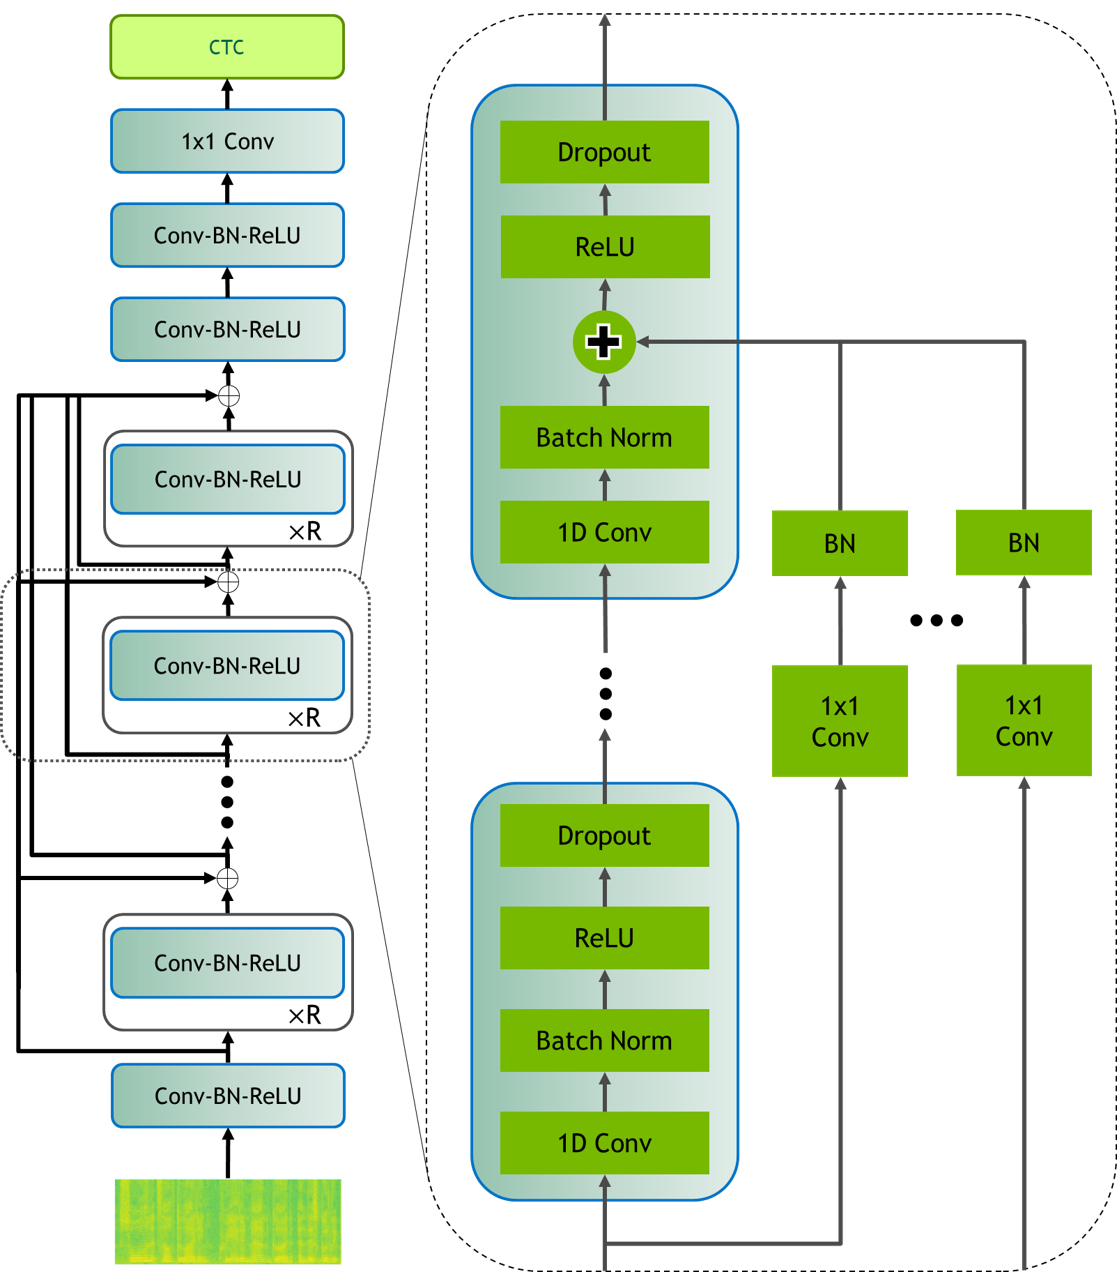
\includegraphics[scale=0.7]{img/JasperVerticalDR4.png}
	\caption{Jasper Dense Residual, taken from \perscite{li2019jasper}.}
	\label{fig:jasper_dr}
\end{figure}

\subsection{QuartzNet}

QuartzNet \parcite{kriman2019quartznet} is another end-to-end ASR architecture used in our work. QuartzNet is a convolutional neural network based on Jasper \parcite{Li2019} architecture having a fraction of parameters (18.9 million versus 333 million) while still achieving near state-of-the-art accuracy.

Same as the Jasper model, the network's input is 64 MFCC features computed from windows of length 20 ms and overlap 10 ms. The network outputs probability over the given alphabet for each time frame. For training is used CTC loss and for decoding beam search.

The main difference between the model and Jasper is the application of 1D time-channel separable convolutions.  Such convolutions can be separated into 1D depthwise convolutional layers with kernel $K$ and a pointwise convolution operating on each time frame independently. Because of this separation, the model has fewer parameters and can even have $3 \times$ larger kernel than the bigger Jasper model.

A further reduction of weights can be achieved by using grouped pointwise convolution instead of the pointwise convolution layer (see  \cref{fig:quartz_arch_groups}). When using four groups, the number of parameters is halved (for QuartzNet-15x5 from 18.9M to 8.7M) with slightly worse performance (WER 3.98 increases to 4.29 for LibriSpeech dev clean and 11.58 increases to 13.48).

As the first described weights reduction is sufficient for our purposes, we work with QuertzNet without the grouped pointwise convolution.

\begin{figure}[h]
	\centering
	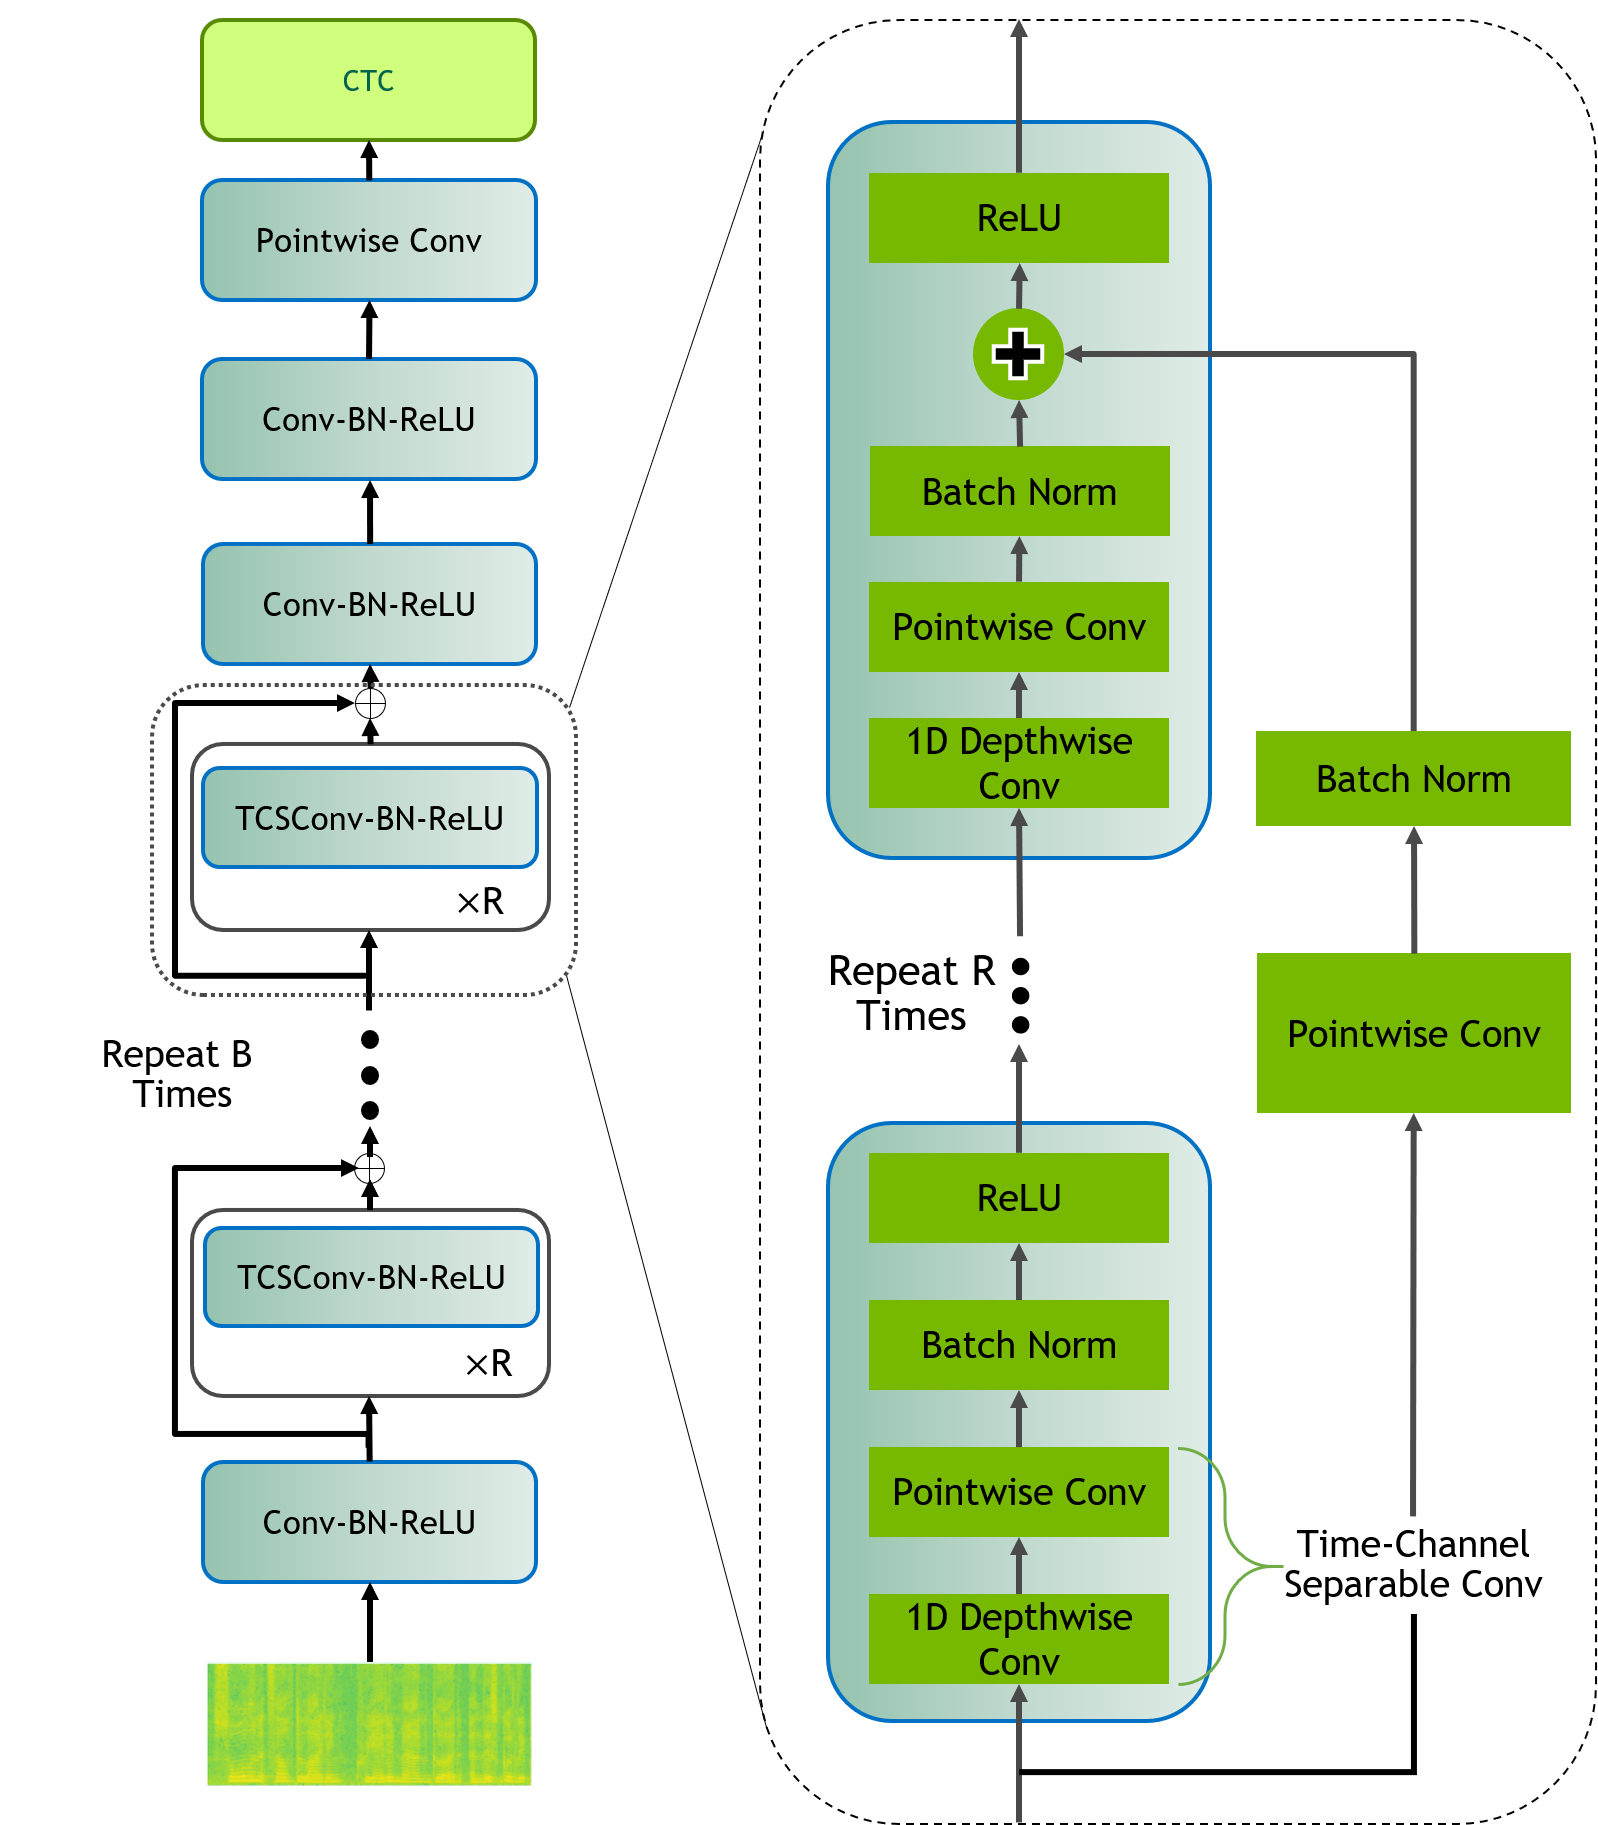
\includegraphics[width=\linewidth]{img/QuartzNet_v2.png}
	\caption{QuartzNet BxR architecture. Taken from \perscite{kriman2019quartznet}.}
	\label{fig:quartz_arch}
\end{figure}

\begin{figure}[h]
	\centering
	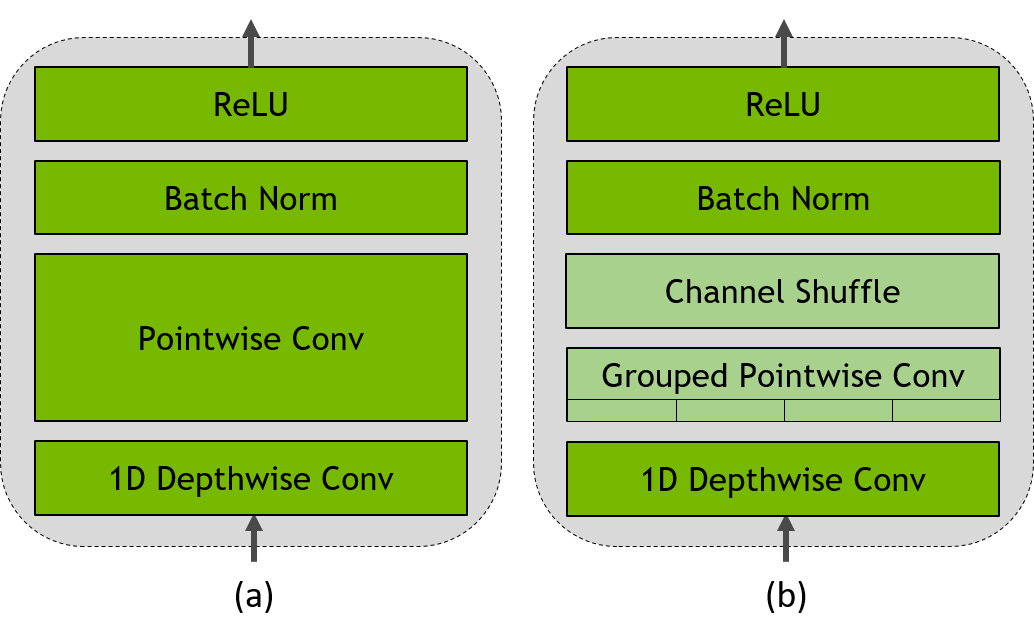
\includegraphics[width=0.8\linewidth]{img/QuartzNet_Grouped_v2.png}
	\caption{(a) Time-channel separable 1D convolutional module (b) Time-channel separable 1D convolutional module with groups and shuffle. Taken from \perscite{kriman2019quartznet}.}
	\label{fig:quartz_arch_groups}
\end{figure}


\subsection{Transformer}
Transformer \parcite{vaswani2017attention} has become a very good established architecture in Neural Machine Translation \parcite{bojar2018proceedings,barrault2019findings}. The main idea behind the architecture is to get rid of recurrence and convolutions and rather base the model solely on attention. As the attention mechanism is implemented as matrix multiplications, contemporary GPUs can better parallelize the computations leading to faster training.

A Transformer model is composed of encoder and decoder (see \cref{fig:transformer}). Both encoder and decoder are stacked identical layers. Encoder layer has two sub-layers: a multi-head self-attention layer and a fully connected feed-forward network. Decoder layer has extra multi-head attention sub-layer, which performs attention over the output of the encoder. This additional layer is between the self-attention and the feed-forward layers. Self-attention in the decoder is modified so that the auto-regressive property holds, i.e., the encoder cannot look to the right side (``future'').

The advantage of self-attention is that it can access arbitrary position in a constant number of sequentially executed operations while recurrent networks need $O(n)$ sequentially executed operations. If the sequence length is less than the representation dimension, which is often the case, the total computational complexity is lower than of the recurrent models. Another advantage presented by the authors is that self-attention leads to better interpretable models. They claim the individual attention heads seem to learn some specific functions that may be related to the syntactic and semantic structure of a sentence.

We employ this model in our enhanced ASR pipeline as a correction and language model and as a translation model in our SLT pipeline. 

\begin{figure}[h]
	\centering
	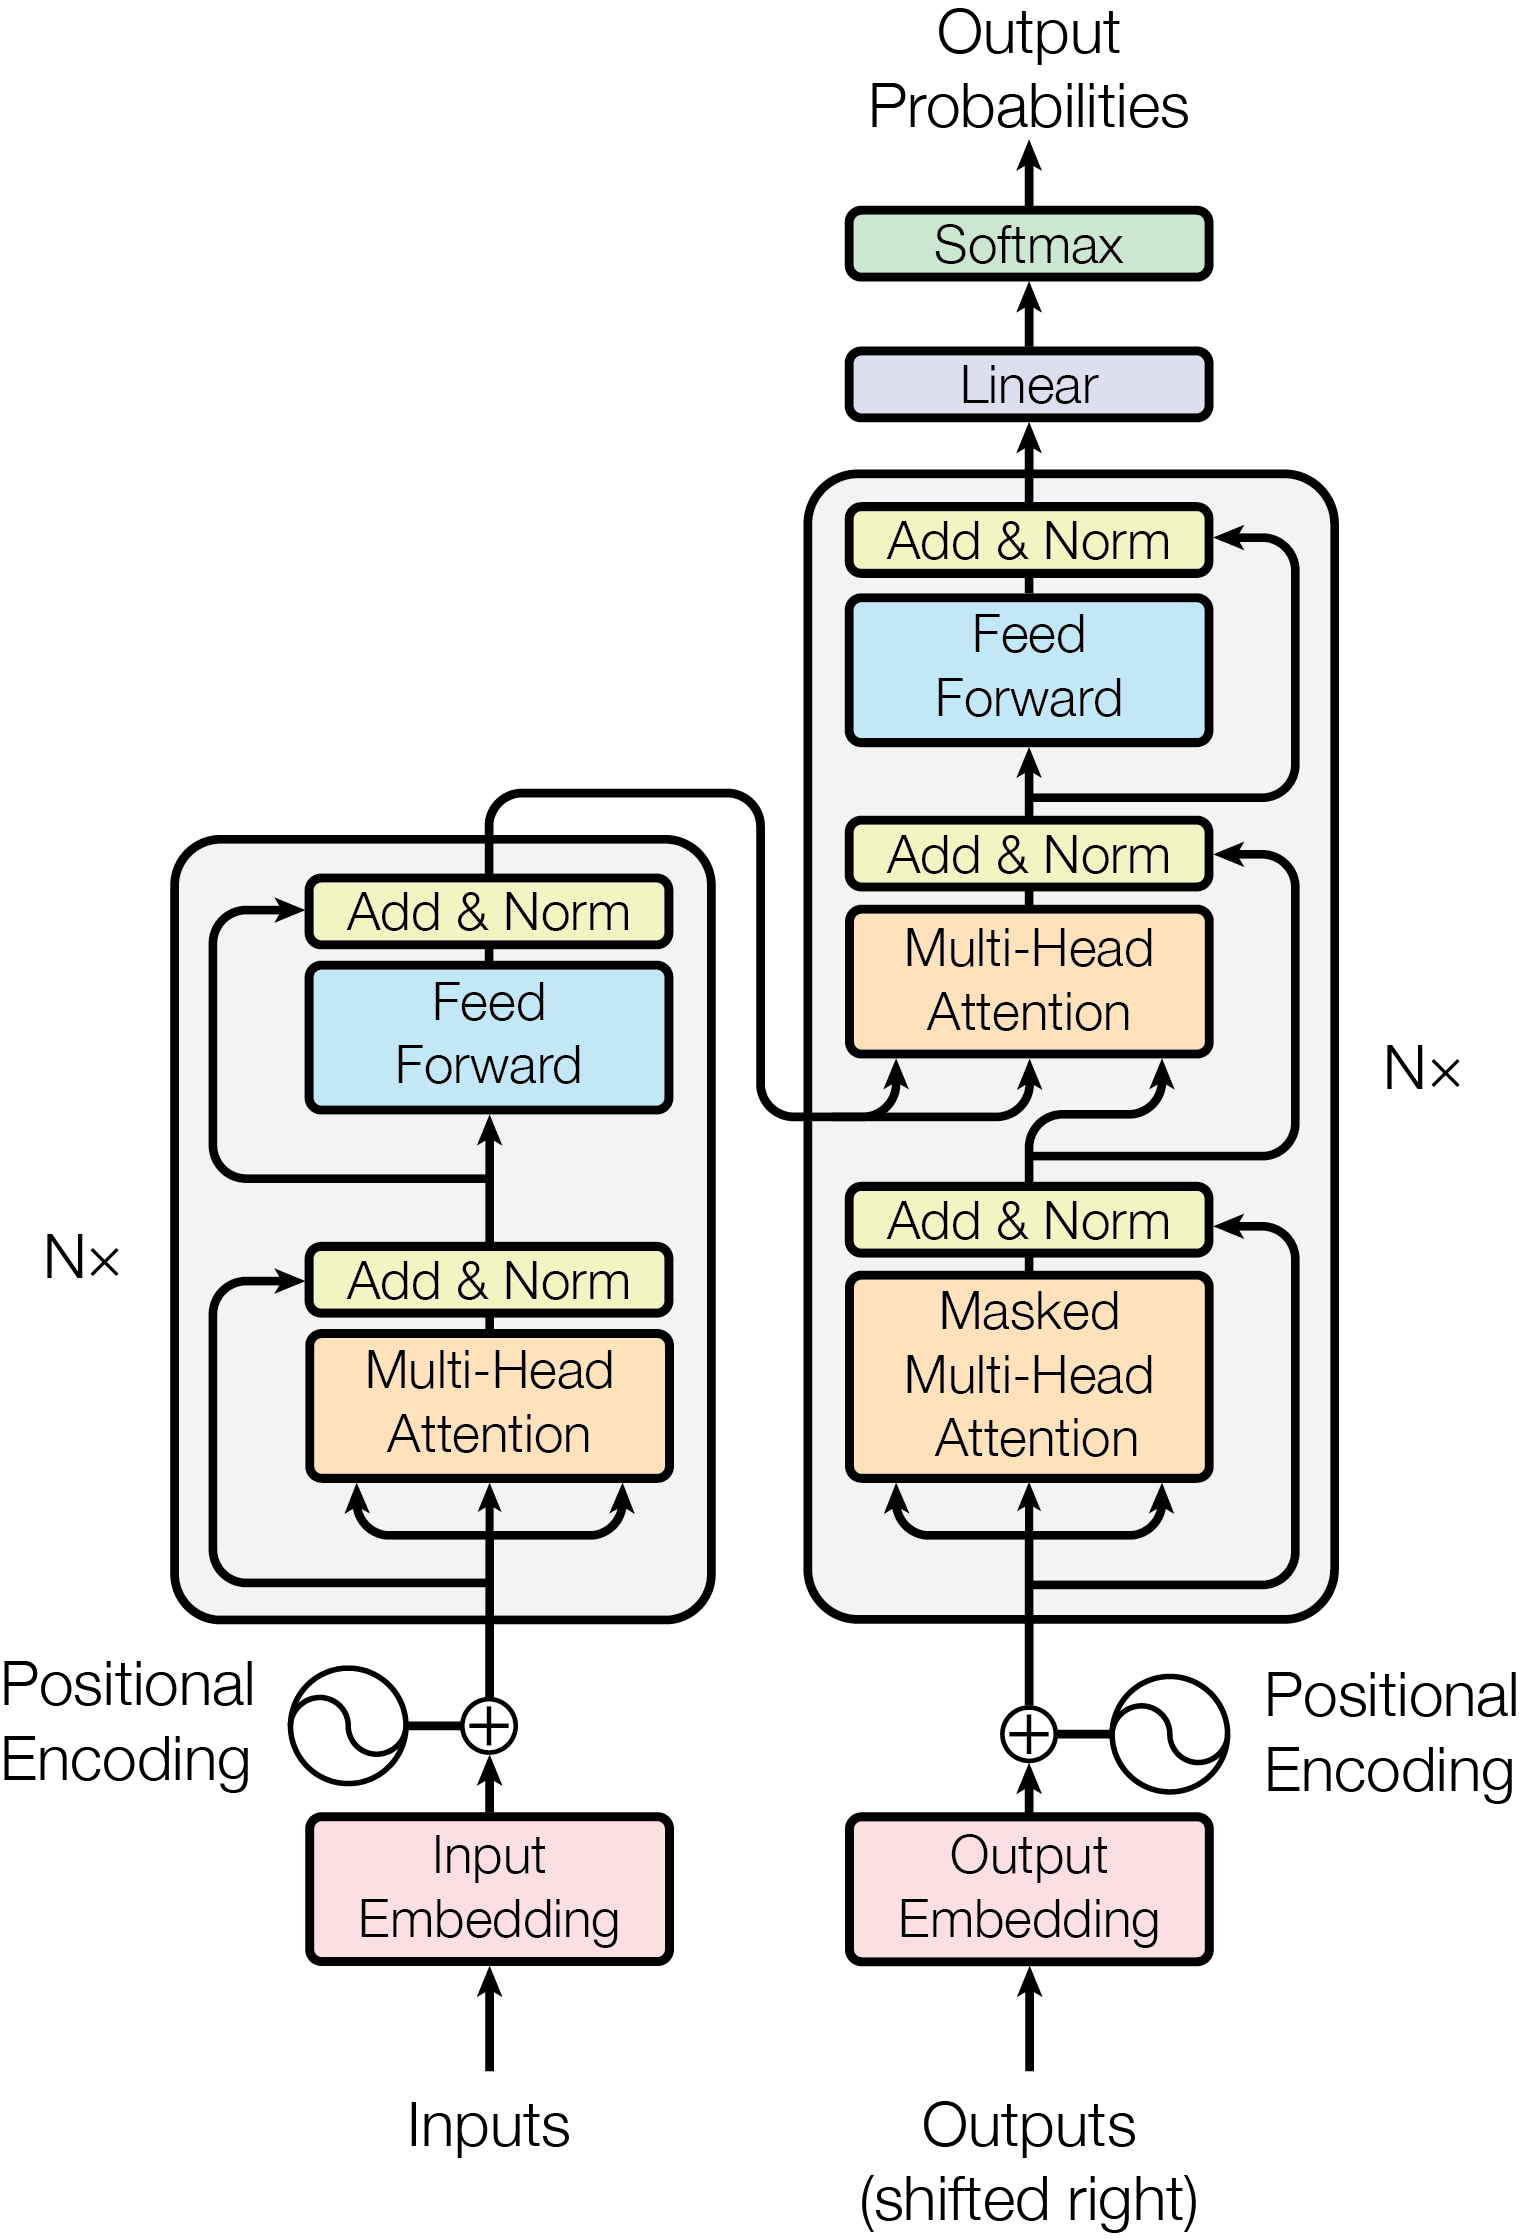
\includegraphics[width=0.8\linewidth]{img/ModalNet-21.png}
	\caption{Transformer model architecture with detailed encoder (left) and decoder (right). Taken from \perscite{vaswani2017attention}}
	\label{fig:transformer}
\end{figure}

\section{Data representation}
This section introduces to the reader the data representations. The way how we encode and feed the neural network can significantly influence performance. In this work, we transcribe recordings, i.e., we work with voice and text data. First, we introduce MFCC --- the voice presentation, and then we discuss text encoding.

\subsection{MFCC}
\label{mfcc}
Mel frequency cepstral coefficiets (MFCC) is the most commonly used representation of speech for ASR and SLT. 
This method exploits the way how the human auditory system perceives voice. Filter in the MFCC pipeline is linearly spaced for frequencies up to 1000 Hz and logarithmically above. 

MFCC pipeline as described in \perscite{muda2010voice} and \perscite{kamath2019deep}:

\begin{enumerate}
	\litem{Pre-emphasis} Application of filter that emphasises higher frequencies:
	
	\begin{equation}
	Y[n] = X[n] - \alpha X[n-1]
	\end{equation}.
	
	This filter makes the signal less dependent on strong signals from previous time steps.
	
	\litem{Framing} Raw audio is segmented into small windows. Signal in small windows can be then treated as stationary. Typically, the length of the window is about 20 ms, and windows have an overlap of 10 ms.
	
	\litem{Windowing} To avoid potential abrupt changes caused by framing windowing is applied. Windowing is a multiplication of samples in a window with a scaling function. Most commonly used in ASR is Hann and Hamming windowing:
	\begin{equation}
	w(n) = \sin^2{\left( \frac{\pi n}{N - 1} \right)}
	\end{equation}
	\begin{equation}
	w(n) = 0.54 - 0.46 \cos{\left(\frac{2\pi n}{N - 1}\right)}
	\end{equation}
	where $N$ is window length and $0 \leq n \leq N - 1$.
	
	\litem{Fast Fourier Transform} FFT converts one-dimensional signal from time to frequency domain.
	
	\litem{Mel Filter Bank}
	The Mel Filter Bank is a set of filters that mimic the human auditory system. Usually, 40 filters are used. Each filter is of a triangular shape. These are used to compute a weighted sum of spectral filter components approximating the Mel scale.
	Each filter output is then the sum of its filtered spectral components. 
	
	\litem{Discrete Cosine Transform} This process converts the log Mel spectrum into a time domain. The result is called the Mel Frequency Cepstrum Coefficient (the MFCC), and the set of coefficients is called acoustic vectors.
\end{enumerate}

An example of a mel-spectrogram is in the \cref{fig:mel}.

\begin{figure}[h]
	\centering
	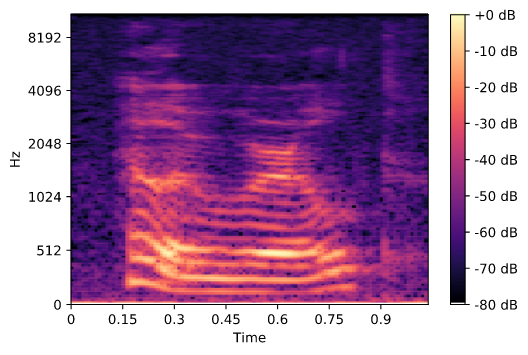
\includegraphics[width=0.8\linewidth]{img/mel.png}
	\caption{Mel spectogram of ``Hello World!''.}
	\label{fig:mel}
\end{figure}

\subsection{Text representation in NMT}

There are many approaches to text representation in NMT. Each of these representations has its advantages and drawbacks. We differentiate the following representations:

\begin{itemize}
	\item character,
	\item word,
	\item sub-word level representation.
\end{itemize}

The first one is a very simple and straightforward approach. Character representation permits one to encode any word (written in given characters). Its downside is that it produces longer sequences compared with other methods. Less output classes lead to the reduction of computational complexity. However, the model needs to attend more positions, which substantially increases time complexity during decoding.

Word level representation, on the other hand, produces shorted sequences. It may be better in some applications as the encoded string is shorter compared with the character-level approach. Generally, though, neural machine translation is an open-vocabulary problem. Word-level representation is undesirable, as it cannot handle unknown words. Several techniques have been proposed, such as NMT with post-processing step \parcite{luong2014addressing,luong2016achieving}.

The most versatile method seems to be a sub-word representation. It addresses both problems, as it produces shorter sequences compared, and is also capable of handling unknown and rare words. The number of contemporary NMTs that use sub-word level representation demonstrates its utility. The most prominent sub-word level tokenizers are BPEs \parcite{sennrich2016neural} and subword regularization \perscite{kudo2018subword}. Both methods are based on similar ideas --- they produce more compact text representations. The former is based on the ``merge'' operation that joins the most frequent character sequences together, while the latter is based on unigram language model. A particular benefit of the subword regularization is that it is also able to produce different segmentation.

In our work, we use BPE implementation YouTokenToMe\footnote{\url{https://github.com/VKCOM/YouTokenToMe}}. We chosen this particular implementation as it supports multithreading is considerably faster than other implementations and has Python and command-line interface. Further, it comes with BPE-dropout \parcite{provilkov2019bpe}. BPE-dropout is an enhancement of traditional BPE, which addresses the deterministic nature of the method. BPE-dropout randomly drops some merges from the BPE merge table, which results in different segmentation. Introducing a noise to the data helps to regularize an NMT model training.

\subsubsection{Byte Pair Encoding}
We would like to point out inconsistency of reporting BPE size in literature. Some authors use terms ``\textit{BPE size}'' and ``\textit{number of merge operations}'' as synonyms, although the actual \textit{BPE size} equals \textit{number of merge operations} plus \textit{characters}. In this work, we use term ``\textit{BPE size}'' as absolute vocabulary size --- including characters. 

\section{Data sets}
We dedicate this section to data sets used for the training of models in our work. First, we introduce speech corpora LibriSpeech and Common Voice, and then we introduce translation corpus CzEng.

\subsection{LibriSpeech}
LibriSpeech \parcite{panayotov2015librispeech} is a large corpus of read English speech. The corpus contains 1000 hours of transcribed speech based on audiobooks from project VoxForge\footnote{\url{http://www.voxforge.org/}}.

The data set is structured into three parts that have approximately 100, 360, and 500 hours. Using a trained model on the Wall Street Journal corpus \parcite{paul1992design}, authors divided the speakers by WER into two pools: ``clean'' and ``other''. From the ``clean'' pool, 20 male and female speakers were randomly selected to development and test sets. The rest was assigned to 100 and 360 hours of ``clean'' sets. For the ``other'' pool (500 hours), authors selected more challenging data for development and test sets.

\subsection{Common Voice}

Common Voice \perscite{ardila2019common} is a multi-lingual, crowdfunded speech corpus. At the time of the writing, 29 languages were available. English data set contained 1118 hours of validated, transcribed recordings. Unfortunately, the Czech data set was not available.

All utterances are collected and validated by volunteers. The data collection runs solely online through a web form. Speech utterances are stored in MPEG-3 format with a 48 kHz sampling rate. After at least two out of three volunteers up-votes an utterance, it is considered to be valid.

The number of clips is divided among the three datasets according to statistical power analyses.  Given the total number of validated clips in a language, the number of clips in the test set is equal to the amount needed to achieve a confidence level of 99\% with a margin of error of 1\% relative to the number of clips in the training set.  The same is true of the development set.

\subsection{Large Corpus of Czech Parliament Plenary Hearings}
Large Corpus of Czech Parliament Plenary Hearings \perscite{dataset} is a corpus of Czech transcribed speech. In our work, we use this dataset for the training of Czech ASR. The corpus has approximately 400 hours. As usual, the dataset contains training, evaluation, and test sets with no overlap. Training and development sets may have some common speakers. The test set should have no speaker overlap with the rest of the corpus.

A notable contrast with other speech corpora is the segmentation. The authors segmented the recordings into short utterances (the longest one has 44s), disregarding the sentences.

\subsection{CzEng 1.7}
Czeng 1.7 is a Czech-English parallel corpus containing about half a billion words. Czeng 1.7 is a filtered version of Czeng 1.6 \parcite{bojar2016czeng}. The advantage of the Czeng corpus is its rich origins such as subtitles, EU legislation, fiction, web pages, technical documents, or medical data. 

\subsubsection{Filtered CzEng}
\label{filtered_czeng}
For our purposes, we distilled out all sentence pairs that ``probably'' do not occur in spoken language. We assume the following: characters, numbers, apostrophe, punctuation, currency sign, dash, and quotation marks on the English side mark the sentence pair as a ``probable'' spoken utterance. Moreover, we filtered out too long and too short sentences (sentences must have at least two characters, at most 511 characters).

We intend to filter out sentences as for example \\

\begin{minipage}{0.95\linewidth}
	\small\emph{E-006961/11 (PL) Marek Henryk Migalski (ECR) to the Commission (15 July 2011)}\\
\end{minipage}


Such utterances do not have straightforward pronunciation, could break \texttt{phone\-mi\-zer}, and could degrade the transcript and translation quality.

\section{Error Metrics}
In this work, we use two error metrics, one for measuring the quality of speech recognition systems --- word error rate (WER) --- and a metric for evaluation of spoken language translation --- BLEU.

\subsection{Word Error Rate}
Word error rate is one of the most commonly used metrics. This metric measures edit distance (insertions, deletions, and substitutions) between target and hypothesis:

\begin{equation}
WER = 100 \times \frac{I + D + S}{N}
\end{equation}

where

\begin{itemize}
	\item $I$ is number of insertions,
	\item $D$ is number of deletions,
	\item $S$ is number of substitutions,
	\item $N$ is number of words in target.
\end{itemize}

Similarly is defined character error rate where, instead of words, are characters considered.

\subsection{BLEU}
For the evaluation of translation tasks, we use BLEU (Bilingual Evaluation Understudy) score introduced by \perscite{papineni2002bleu}. This metric assigns scores in the interval $[0,1]$, where 1 is the perfect score. The method counts occurrences of matching n-grams in candidate and reference (there can be more than one reference translations). It computes a modified n-gram precision (number of occurrences of an n-gram in candidate sentence must not exceed the maximum number of occurrences in any reference, otherwise is clipped) and does a weighted geometric mean. In addition to the implicit penalization of length, the metric introduces the brevity penalty.

Usage of this metric used to lead to confusion previously because its actual implementation could vary. We therefore use in our work \texttt{SacreBLEU} proposed by \perscite{post2018call}.